\nocite{*}
\bibliographystyle{apalike}
\bibliography{references}

\appendix


\section{Test Cases}

\begin{table}[H]
    \begin{tabular}{ll}
    \hline
    \textbf{Query}       & \textbf{Target}                                    \\
    \hline
    NVIDIA 研替 & NVIDIA 2025 研發替代役/實習開放職缺資訊                \\
    114甄試     & 114學年度碩士班甄試入學第2階段備取生名單及報到注意事項             \\
    甄試名單    & 114學年度碩士班甄試入學第1階段                         \\
    AI競賽      & AI Junior Award 2025                      \\
    書卷獎       & 【學士班】112學年度第2學期書卷獎得獎名單公告                  \\
    導師名單      & 113.10.15更新【學士班】113學年度第一學期大學部導生名單         \\
    特殊選材      & 114學年度資訊工程學系特殊選才招生公告                      \\
    畢業學分      & 【學士班】113學年度資工系學士班「畢業學分預審」作業公告(請於10/11前繳交) \\
    校友 頒獎     & 資訊人院刊- 資訊系友【交大日資工系友回娘家暨傑出系友頒獎典禮】          \\
    學士畢業      & 【學士班】資訊工程學系畢業離系/離校作業公告                   \\
    \hline
    \end{tabular}
\end{table}

\section{A Deep Dive into Word Vector Implementations}
\subsection{Word Representation}
The foundation of all NLP tasks lies in how we represent words as inputs for models. Traditionally, words were treated as distinct symbols. However, to excel in NLP, we need to capture the similarities and differences between words. Word vectors effectively encode these relationships, often utilizing measures like Cosine or Euclidean distance to quantify similarity.

\subsection{Word Vectors}
The English language comprises approximately 13 million tokens, but not all are unrelated. To handle this complexity, we encode words into vectors that occupy points in a "word space." This approach assumes an N-dimensional space can encapsulate the semantics of language, where each dimension conveys specific meanings such as tense (past, present, future), count (singular, plural), or gender (masculine, feminine).

\subsubsection{One-Hot Vectors}
The simplest form of word vector is the one-hot vector, where each word is represented as an $R^{\left| V \right| \times 1}$ vector, with a single $1$ at the index corresponding to the word in the sorted vocabulary. For example:

\begin{equation*}
w^{\text{aardvark}} = 
\begin{bmatrix}
1 \\
0 \\
0 \\
\vdots \\
0
\end{bmatrix}
,\ 
w^{\text{a}} = 
\begin{bmatrix}
0 \\
1 \\
0 \\
\vdots \\
0
\end{bmatrix}
,\ 
w^{\text{at}} = 
\begin{bmatrix}
0 \\
0 \\
1 \\
\vdots \\
0
\end{bmatrix}
,\ 
\cdots
,\ 
w^{\text{zebra}} = 
\begin{bmatrix}
0 \\
0 \\
0 \\
\vdots \\
1
\end{bmatrix}
\end{equation*}

In this encoding, words are treated as independent entities, offering no insight into similarity. For instance: 

\begin{equation*}
    (w^{\text{hotel}})^{T}w^{\text{motel}} = (w^{\text{hotel}})^{T}w^{\text{cat}} = 0
\end{equation*}

This approach, termed denotational semantics, is sparse and fails to capture relationships or similarities between words.

\subsubsection{Reducing Dimensionality}
To better encode relationships, we can reduce the dimensionality of the representation from $\Bbb{R}^{\left| V \right|}$ to a smaller subspace.



\subsection{SVD-Based Methods}
To generate word embeddings, we analyze word co-occurrences in a dataset, creating a matrix $X$. Singular Value Decomposition (SVD) is then applied to $X$, yielding a $USV^{T}$ decomposition. Rows of $U$ serve as word embeddings. Below are key approaches to constructing $X$:

\subsubsection{Word-Document Matrix}
Assuming related words frequently appear in the same documents, we construct $X$ by counting occurrences of word $i$ in document $j$. Although effective, this results in a large, sparse $\Bbb{R}^{\left| V \right| \times M}$ matrix, where $M$ is the document count.

\subsubsection{Window-Based Co-occurrence Matrix}
Here, $X$ captures word co-occurrence within a fixed window size. For example, using a corpus of three sentences and a window size of 1:
\begin{enumerate}
    \item I enjoy flying.
    \item I like NLP.
    \item I like deep learning.
\end{enumerate}
The resulting $X$ matrix shows co-occurrence counts.

\begin{equation}
X=
\kbordermatrix{
                & I    & like & enjoy & deep & learning & NLP & flying & . \\
    I          & 0    & 2    & 1     & 0    & 0        & 0   & 0      & 0 \\
    like       & 1    & 0    & 0     & 1    & 0        & 1   & 0      & 0 \\
    enjoy      & 3    & 4    & 3     & 0    & 0        & 0   & 0      & 0 \\
    deep       & 0    & 0    & 0     & 2    & 8        & 0   & 1      & 0 \\
    learning   & 0    & 0    & 0     & 3    & 7        & 0   & 0      & 0 \\
    NLP        & 0    & 4    & 1     & 0    & 0        & 2   & 3      & 0 \\
    flying     & 0    & 0    & 1     & 0    & 3        & 1   & 5      & 0 \\
    .          & 0    & 0    & 0     & 0    & 0        & 0   & 0      & 1
}
\end{equation}

\subsubsection{Applying SVD}
SVD decomposes $X$, and a cutoff $k$ is selected to retain a specified variance:
\begin{equation}
    \frac{ {\textstyle \sum_{i=1}^{k}} \sigma _i}{ {\textstyle \sum_{i=1}^{\left| V \right|}} \sigma _i}
\end{equation}

This yields a k-dimensional representation for each word.
Applying SVD to $X$:

\begin{equation}
\begin{gathered}
\left| V \right| 
\overset{\left| V \right|}{
\left[
    \begin{array}{ccc}
        &   &   \\
        & \hat{X} &   \\
        &   &  
    \end{array}
\right]
}
=
\left| V \right|
\overset{\left| V \right|}{
\left[
    \begin{array}{ccc}
        \mid  & \mid &   \\
        u_1   & u_2  & \cdots  \\
        \mid  & \mid &  
    \end{array}
\right]
}
\ \left| V \right| \ 
\overset{\left| V \right|}{
\left[
    \begin{array}{ccc}
        \sigma_1 & 0        & \cdots \\
        0        & \sigma_2 & \cdots \\
        \vdots   & \vdots   & \ddots
    \end{array}
\right]
}
\ \left| V \right| \ 
\overset{\left| V \right|}{
\left[
    \begin{array}{ccc}
        - & v_1 & - \\
        - & v_2 & - \\
            & \vdots &  
    \end{array}
\right]
}
\end{gathered}
\end{equation}

Reducing dimensionality by selecting first k singular vectors:

\begin{equation}
\begin{gathered}
\left| V \right| 
\overset{\left| V \right|}{
\left[
    \begin{array}{ccc}
        &   &   \\
        & \hat{X} &   \\
        &   &  
    \end{array}
\right]
}
=
\left| V \right|
\overset{k}{
\left[
    \begin{array}{ccc}
        \mid  & \mid &   \\
        u_1   & u_2  & \cdots  \\
        \mid  & \mid &  
    \end{array}
\right]
}
\ k \ 
\overset{k}{
\left[
    \begin{array}{ccc}
        \sigma_1 & 0        & \cdots \\
        0        & \sigma_2 & \cdots \\
        \vdots   & \vdots   & \ddots
    \end{array}
\right]
}
\ k \ 
\overset{\left| V \right|}{
\left[
    \begin{array}{ccc}
        - & v_1 & - \\
        - & v_2 & - \\
            & \vdots &  
    \end{array}
\right]
}
\end{gathered}
\end{equation}

\subsubsection{Challenges with SVD Methods}
While SVD methods encode semantic and syntactic relationships, they face several issues:
\begin{itemize}
    \item Frequent changes in vocabulary and corpus size
    \item High computational cost
    \item Sparsity and high dimensionality
    \item Inefficiency in adding new words
\end{itemize}

\subsection{Iterative Methods: Word2Vec}
To address these challenges, iterative methods like Word2Vec focus on learning word vectors incrementally. Instead of relying on a global matrix, Word2Vec trains a model on smaller objectives, learning word representations through iterative updates. It employs two algorithms:
\begin{itemize}
    \item \textbf{Continuous Bag-of-Words (CBOW)}: Predicts a center word from its surrounding context.
    \item \textbf{Skip-Gram}: Predicts context words given a center word.
\end{itemize}

Two training techniques are used:
\begin{itemize}
    \item \textbf{Negative Sampling}: Optimizes an objective by sampling non-context words.
    \item \textbf{Hierarchical Softmax}: Uses a tree structure for efficient probability computation.
\end{itemize}

This method leverages distributional similarity—the idea that words appearing in similar contexts are likely to have similar meanings. Word2Vec’s simplicity and scalability make it a significant advancement in word embedding techniques.

\section{Screenshots}

\includegraphics[width=\textwidth]{screenshots/sc1.jpeg}
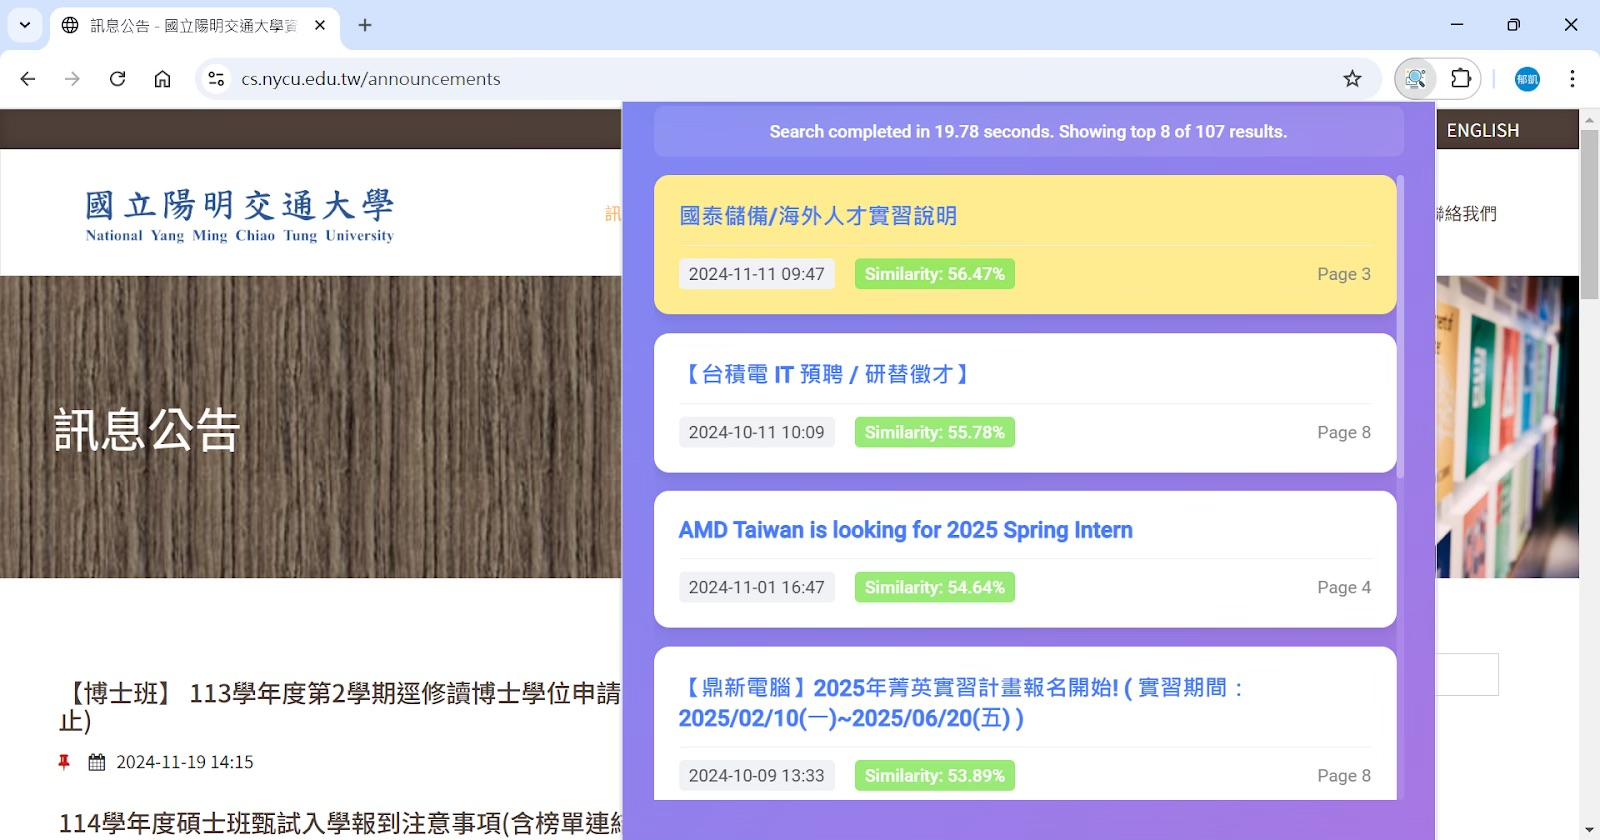
\includegraphics[width=\textwidth]{screenshots/sc2.jpeg}

\includegraphics[width=\textwidth]{screenshots/sc3.jpeg}

\includegraphics[width=\textwidth]{screenshots/sc4.jpeg}
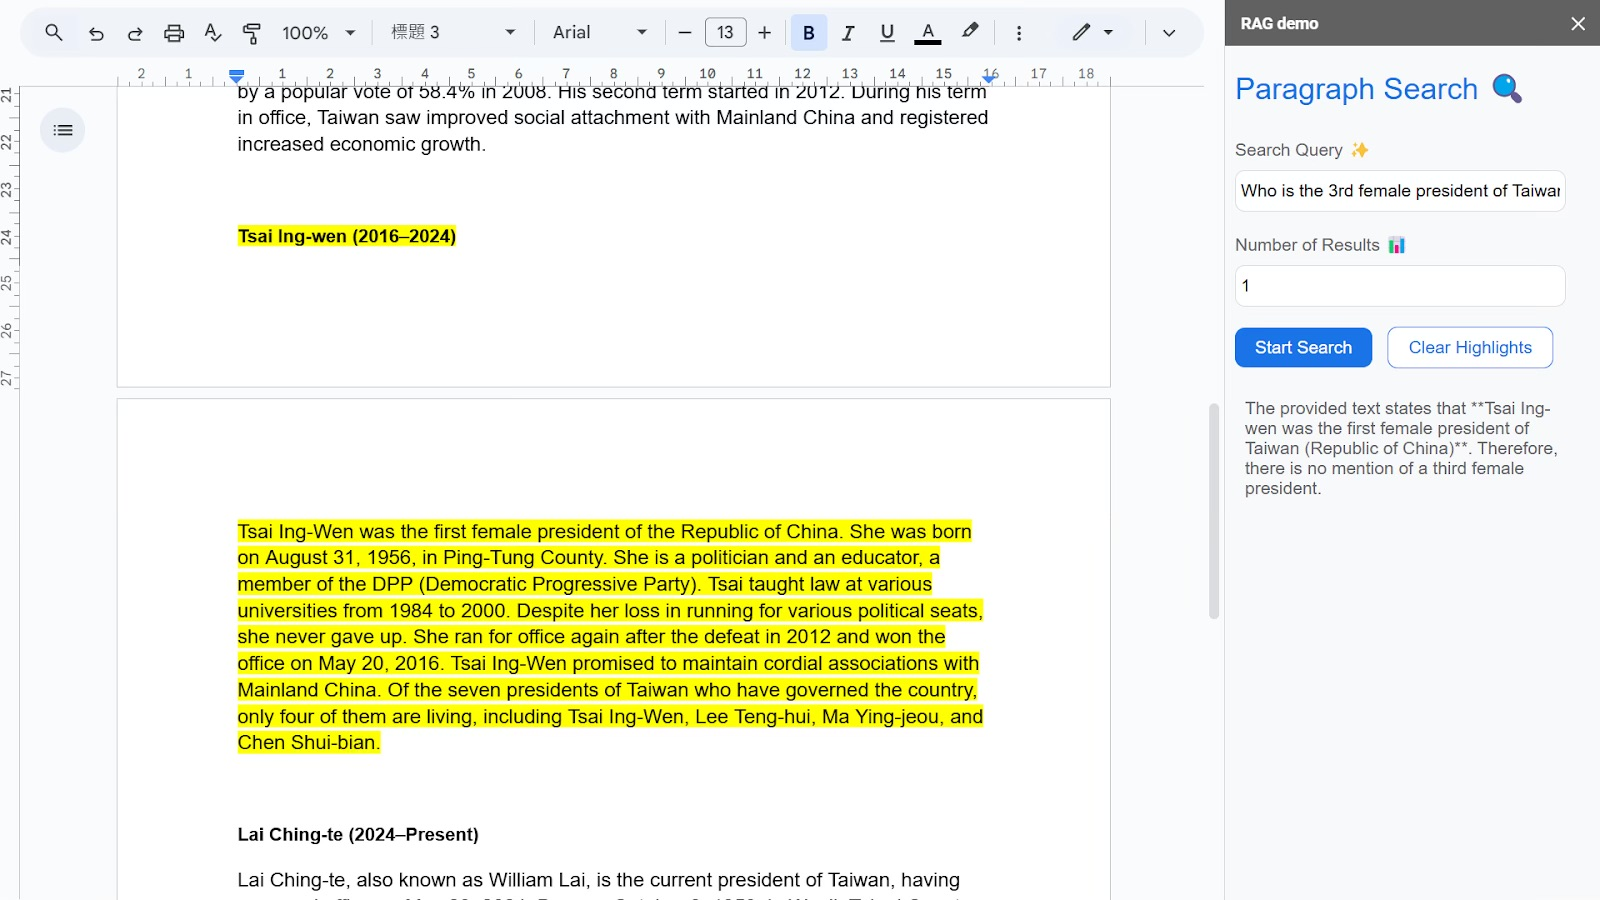
\includegraphics[width=\textwidth]{screenshots/rag1.jpeg}
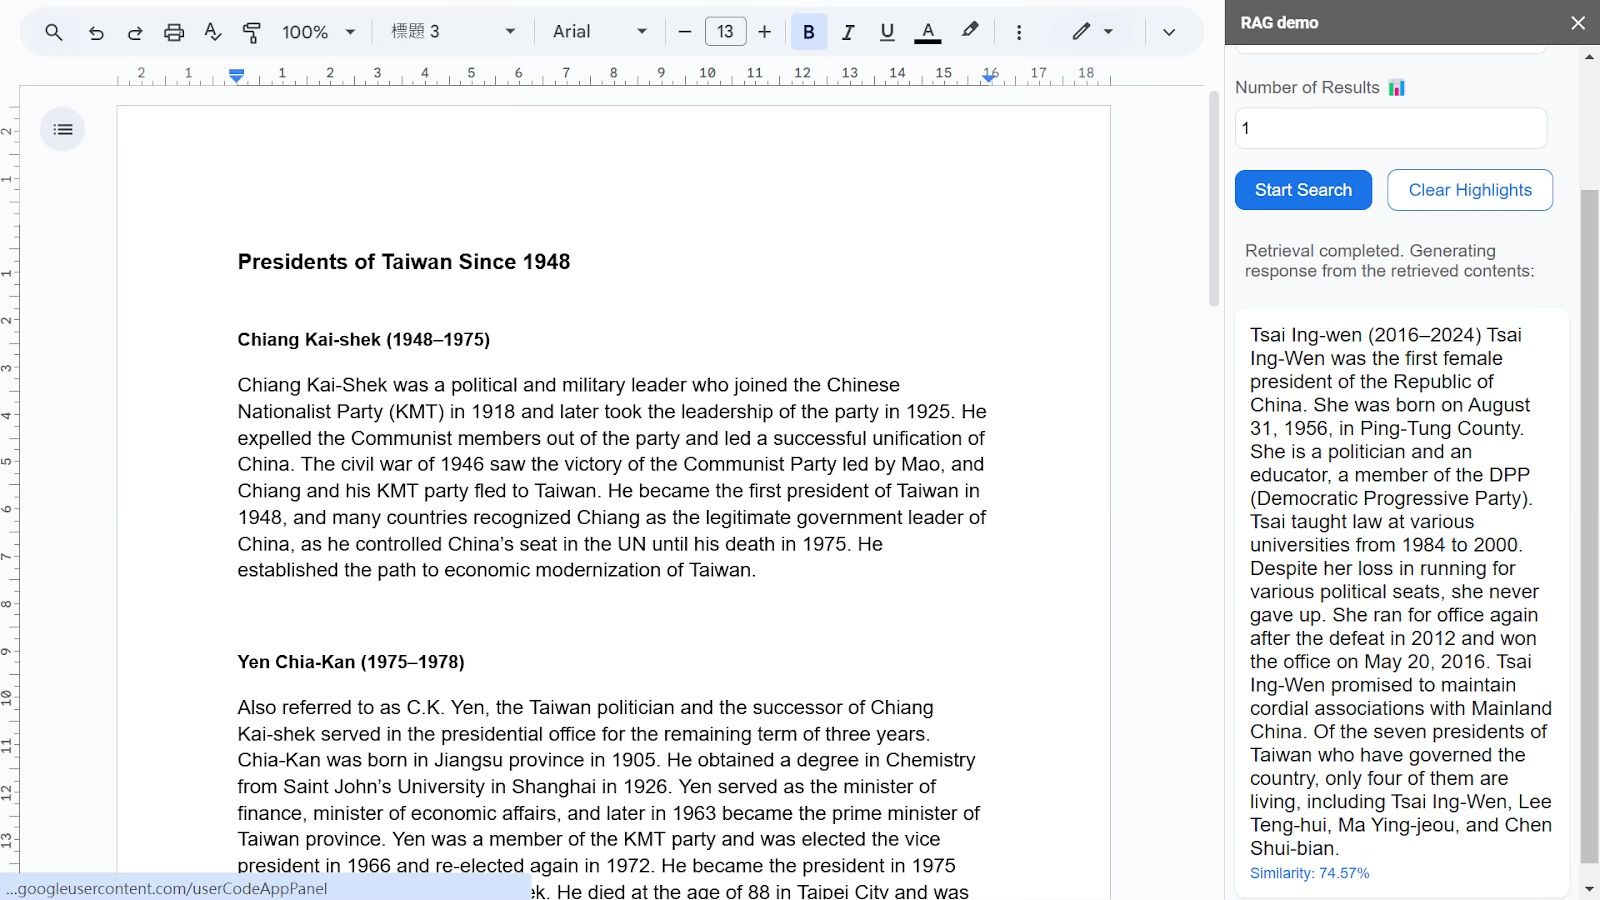
\includegraphics[width=\textwidth]{screenshots/rag2.jpeg}
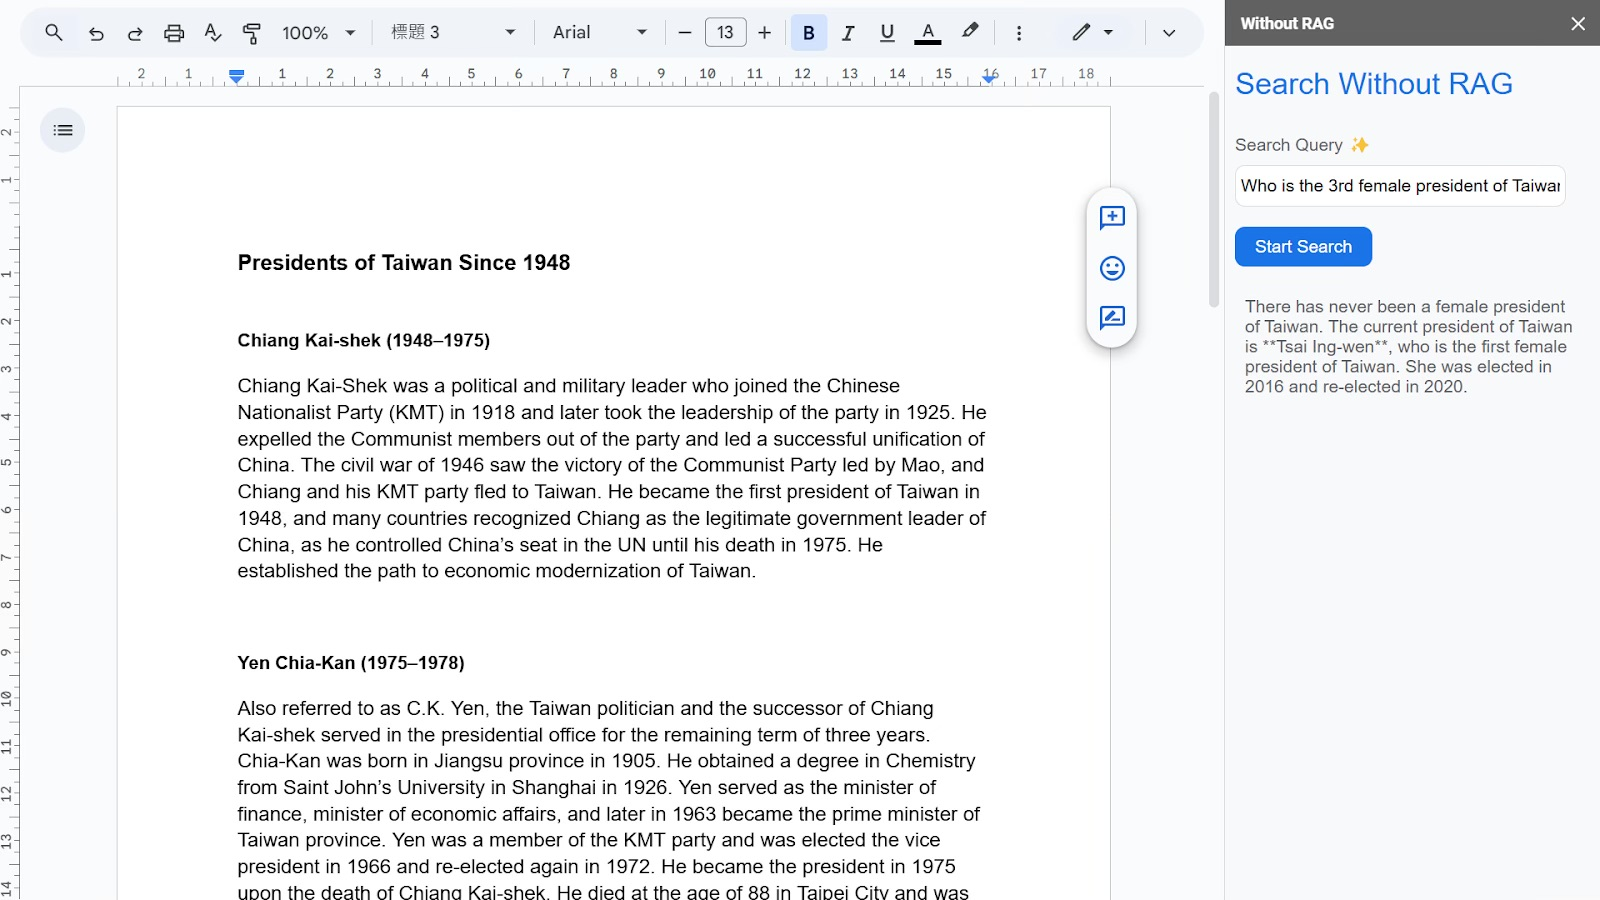
\includegraphics[width=\textwidth]{screenshots/rag3.jpeg}


\section{Code Implementation}


\small
\begin{lstlisting}
import requests
from bs4 import BeautifulSoup
from tqdm import tqdm
from googletrans import Translator
from nltk.tokenize import word_tokenize
from nltk.corpus import stopwords
import numpy as np
from sentence_transformers import SentenceTransformer
from sklearn.metrics.pairwise import cosine_similarity


# Article class definition
class Article:
    def __init__(self, url: str, title: str) -> None:
        self.article_url = url
        self.original_title = title
        self.translated_title = ""

class ArticleCollection:
    def __init__(self):
        self.articles = []

    def add_article(self, article: Article):
        self.articles.append(article)

    def display_titles(self):
        for article in self.articles:
            print(f"Original Title: {article.original_title}")
            print(f"URL: {article.article_url}")
            print("-" * 15)


class ArticleCollectionFromUrl(ArticleCollection):
    def __init__(self, urls=[]):
        super().__init__()
        self.urls = urls

    def fetch_articles(self):
        for url in tqdm(self.urls):
            response = requests.get(url)
            if response.status_code == 200:
                soup = BeautifulSoup(response.text, "html.parser")
                for item in soup.find_all("li", class_="announcement-item"):
                    link_tag = item.find("h2").find("a")
                    title = link_tag.text.strip()
                    href = link_tag["href"]
                    self.add_article(Article(url=href, title=title))
            else:
                print(f"Unable to access site, status code: {response.status_code}")


# Article translation function
translator = Translator()

def translate_articles(articles):
    for article in tqdm(articles):
        article.translated_title = translator.translate(article.original_title, dest="en").text


# Article search functionality
class ArticleSearch:
    def __init__(self, articles):
        self.articles = articles
        self.model = SentenceTransformer("all-mpnet-base-v2")
        self.article_titles = [article.translated_title for article in articles]
        self.article_vectors = self.model.encode(self.article_titles)

    def search(self, query):
        query_vector = self.model.encode([query])
        similarities = np.array([cosine_similarity(query_vector, vector)[0][0] for vector in self.article_vectors])
        return similarities

    def print_suggestions(self, query, k=5):
        similarities = self.search(query)
        suggestions = np.argsort(-similarities)[:k]
        for idx in suggestions:
            print(f"{similarities[idx]:.4f} : {self.articles[idx].translated_title}")
            print(f"\t\t {self.articles[idx].article_url}")
        print(f"Most similar article: {self.articles[suggestions[0]].translated_title}")


# Translate test query
def translate_test_query(test_cases):
    for test_case in test_cases:
        test_case.query = translator.translate(text=test_case.query, dest="en").text


class TestCase:
    def __init__(self, query, target):
        self.query = query
        self.target = target
    
    def get_score(self, article_search):
        similarities = article_search.search(self.query)
        target_idx = next((i for i, article in enumerate(article_search.articles) if self.target in article.original_title), None)
        if target_idx is None:
            return 0
        most_similar_idx = np.argsort(-similarities)
        return 1 / (np.where(most_similar_idx == target_idx)[0][0] + 1) if target_idx in most_similar_idx else 0


# Main program
PAGES = 1
articles = ArticleCollectionFromUrl([f"https://www.cs.nycu.edu.tw/announcements?page={i}" for i in range(1, PAGES+1)])
articles.fetch_articles()
translate_articles(articles.articles)

# Article search
article_search = ArticleSearch(articles.articles)
article_search.print_suggestions("NVIDIA 研替", k=5)

# Define Test Cases (not all of them are shown)
test_cases = [
    TestCase("AI競賽", "AI Junior Award 2025")
]

# Evaulation
def runtest():
    scores = sum([test_case.get_score(article_search) for test_case in test_cases]) / len(test_cases)
    print(f"score: {scores:.3f}")

runtest()
\end{lstlisting}

\section{Training code}
\begin{lstlisting}
import io
import re
import string
import tqdm

import numpy as np
import tensorflow as tf
from tensorflow.keras import layers

# Load the TensorBoard notebook extension
%load_ext tensorboard

# Constants
SEED = 42
AUTOTUNE = tf.data.AUTOTUNE

# Vectorize an example sentence
sentence = "The wide road shimmered in the hot sun"
tokens = list(sentence.lower().split())
print(len(tokens))

# Create a vocabulary
vocab, index = {}, 1
vocab[''] = 0
for token in tokens:
    if token not in vocab:
        vocab[token] = index
        index += 1
vocab_size = len(vocab)
print(vocab)

# Create an inverse vocabulary
inverse_vocab = {index: token for token, index in vocab.items()}
print(inverse_vocab)

# Vectorize the sentence
example_sequence = [vocab[word] for word in tokens]
print(example_sequence)

# Generate skip-grams
window_size = 2
positive_skip_grams, _ = tf.keras.preprocessing.sequence.skipgrams(
    example_sequence, vocabulary_size=vocab_size, window_size=window_size, negative_samples=0
)
print(len(positive_skip_grams))
for target, context in positive_skip_grams[:5]:
    print(f"({target}, {context}): ({inverse_vocab[target]}, {inverse_vocab[context]})")

# Negative sampling for one skip-gram
target_word, context_word = positive_skip_grams[0]
num_ns = 4
context_class = tf.reshape(tf.constant(context_word, dtype="int64"), (1, 1))
negative_sampling_candidates, _, _ = tf.random.log_uniform_candidate_sampler(
    true_classes=context_class,
    num_true=1,
    num_sampled=num_ns,
    unique=True,
    range_max=vocab_size,
    seed=SEED,
    name="negative_sampling"
)
print(negative_sampling_candidates)
print([inverse_vocab[index.numpy()] for index in negative_sampling_candidates])

# Construct one training example
squeezed_context_class = tf.squeeze(context_class, 1)
context = tf.concat([squeezed_context_class, negative_sampling_candidates], 0)
label = tf.constant([1] + [0]*num_ns, dtype="int64")
target = target_word
print(f"target_index : {target}")
print(f"target_word : {inverse_vocab[target_word]}")
print(f"context_indices : {context}")
print(f"context_words : {[inverse_vocab[c.numpy()] for c in context]}")
print(f"label : {label}")

# Generate training data
def generate_training_data(sequences, window_size, num_ns, vocab_size, seed):
    targets, contexts, labels = [], [], []
    sampling_table = tf.keras.preprocessing.sequence.make_sampling_table(vocab_size)
    for sequence in tqdm.tqdm(sequences):
        positive_skip_grams, _ = tf.keras.preprocessing.sequence.skipgrams(
            sequence,
            vocabulary_size=vocab_size,
            sampling_table=sampling_table,
            window_size=window_size,
            negative_samples=0
        )
        for target_word, context_word in positive_skip_grams:
            context_class = tf.expand_dims(
                tf.constant([context_word], dtype="int64"), 1
            )
            negative_sampling_candidates, _, _ = tf.random.log_uniform_candidate_sampler(
                true_classes=context_class,
                num_true=1,
                num_sampled=num_ns,
                unique=True,
                range_max=vocab_size,
                seed=seed,
                name="negative_sampling"
            )
            context = tf.concat([tf.squeeze(context_class, 1), negative_sampling_candidates], 0)
            label = tf.constant([1] + [0]*num_ns, dtype="int64")
            targets.append(target_word)
            contexts.append(context)
            labels.append(label)
    return targets, contexts, labels

# Download text corpus
path_to_file = tf.keras.utils.get_file(
    'shakespeare.txt', 'https://storage.googleapis.com/download.tensorflow.org/data/shakespeare.txt'
)
with open(path_to_file) as f:
    lines = f.read().splitlines()

# Vectorize sentences from the corpus
def custom_standardization(input_data):
    lowercase = tf.strings.lower(input_data)
    return tf.strings.regex_replace(lowercase, '[%s]' % re.escape(string.punctuation), '')

vocab_size = 4096
sequence_length = 10
vectorize_layer = layers.TextVectorization(
    standardize=custom_standardization,
    max_tokens=vocab_size,
    output_mode='int',
    output_sequence_length=sequence_length
)
text_ds = tf.data.TextLineDataset(path_to_file).filter(lambda x: tf.cast(tf.strings.length(x), bool))
vectorize_layer.adapt(text_ds.batch(1024))
inverse_vocab = vectorize_layer.get_vocabulary()
text_vector_ds = text_ds.batch(1024).prefetch(AUTOTUNE).map(vectorize_layer).unbatch()

# Prepare training examples
sequences = list(text_vector_ds.as_numpy_iterator())
targets, contexts, labels = generate_training_data(
    sequences=sequences, window_size=2, num_ns=4, vocab_size=vocab_size, seed=SEED
)

# Configure the dataset
BATCH_SIZE = 1024
BUFFER_SIZE = 10000
dataset = tf.data.Dataset.from_tensor_slices(((targets, contexts), labels))
dataset = dataset.shuffle(BUFFER_SIZE).batch(BATCH_SIZE, drop_remainder=True).cache().prefetch(buffer_size=AUTOTUNE)

# Define the Word2Vec model
class Word2Vec(tf.keras.Model):
    def __init__(self, vocab_size, embedding_dim):
        super(Word2Vec, self).__init__()
        self.target_embedding = layers.Embedding(vocab_size, embedding_dim, name="w2v_embedding")
        self.context_embedding = layers.Embedding(vocab_size, embedding_dim)

    def call(self, pair):
        target, context = pair
        if len(target.shape) == 2:
            target = tf.squeeze(target, axis=1)
        word_emb = self.target_embedding(target)
        context_emb = self.context_embedding(context)
        dots = tf.einsum('be,bce->bc', word_emb, context_emb)
        return dots

# Compile and train the model
embedding_dim = 128
word2vec = Word2Vec(vocab_size, embedding_dim)
word2vec.compile(
    optimizer='adam',
    loss=tf.keras.losses.CategoricalCrossentropy(from_logits=True),
    metrics=['accuracy']
)
tensorboard_callback = tf.keras.callbacks.TensorBoard(log_dir="logs")
word2vec.fit(dataset, epochs=20, callbacks=[tensorboard_callback])

# Save embeddings
weights = word2vec.get_layer('w2v_embedding').get_weights()[0]
with io.open('vectors.tsv', 'w', encoding='utf-8') as out_v, io.open('metadata.tsv', 'w', encoding='utf-8') as out_m:
    for index, word in enumerate(inverse_vocab):
        if index == 0:
            continue
        vec = weights[index]
        out_v.write('\t'.join([str(x) for x in vec]) + "\n")
        out_m.write(word + "\n")



    
\end{lstlisting}